\chapter{Elevating Aermax – First Sprint Enhancements and Integrations}

\section{Introduction}
In this chapter, we cover the first sprint of the Aermax project, focusing on team collaboration and meetings, as well as the key enhancements and features we implemented to improve the platform.

\section{Team Collaboration and Meetings}

\subsection{Daily Standups}
\textbf{Purpose:} Share daily progress, plan the day, and address blockers. \\
\textbf{Structure:} Each team member provides a brief update on:
\begin{itemize}
    \item What they did yesterday.
    \item What they plan to do today.
    \item Any blockers they are facing.
\end{itemize}

\subsection{Retrospectives}
\textbf{Purpose:} Discuss what went well, what didn’t, and identify areas for improvement. \\
\textbf{Outcome:} Action items to enhance future sprints.

\subsection{Client Meetings}
\textbf{Initial Requirements Gathering:} Detailed discussions to understand client needs. \\
\textbf{Ongoing Feedback Sessions:} Regular updates to demonstrate progress and gather feedback.
\begin{figure}[H]
    \centering
    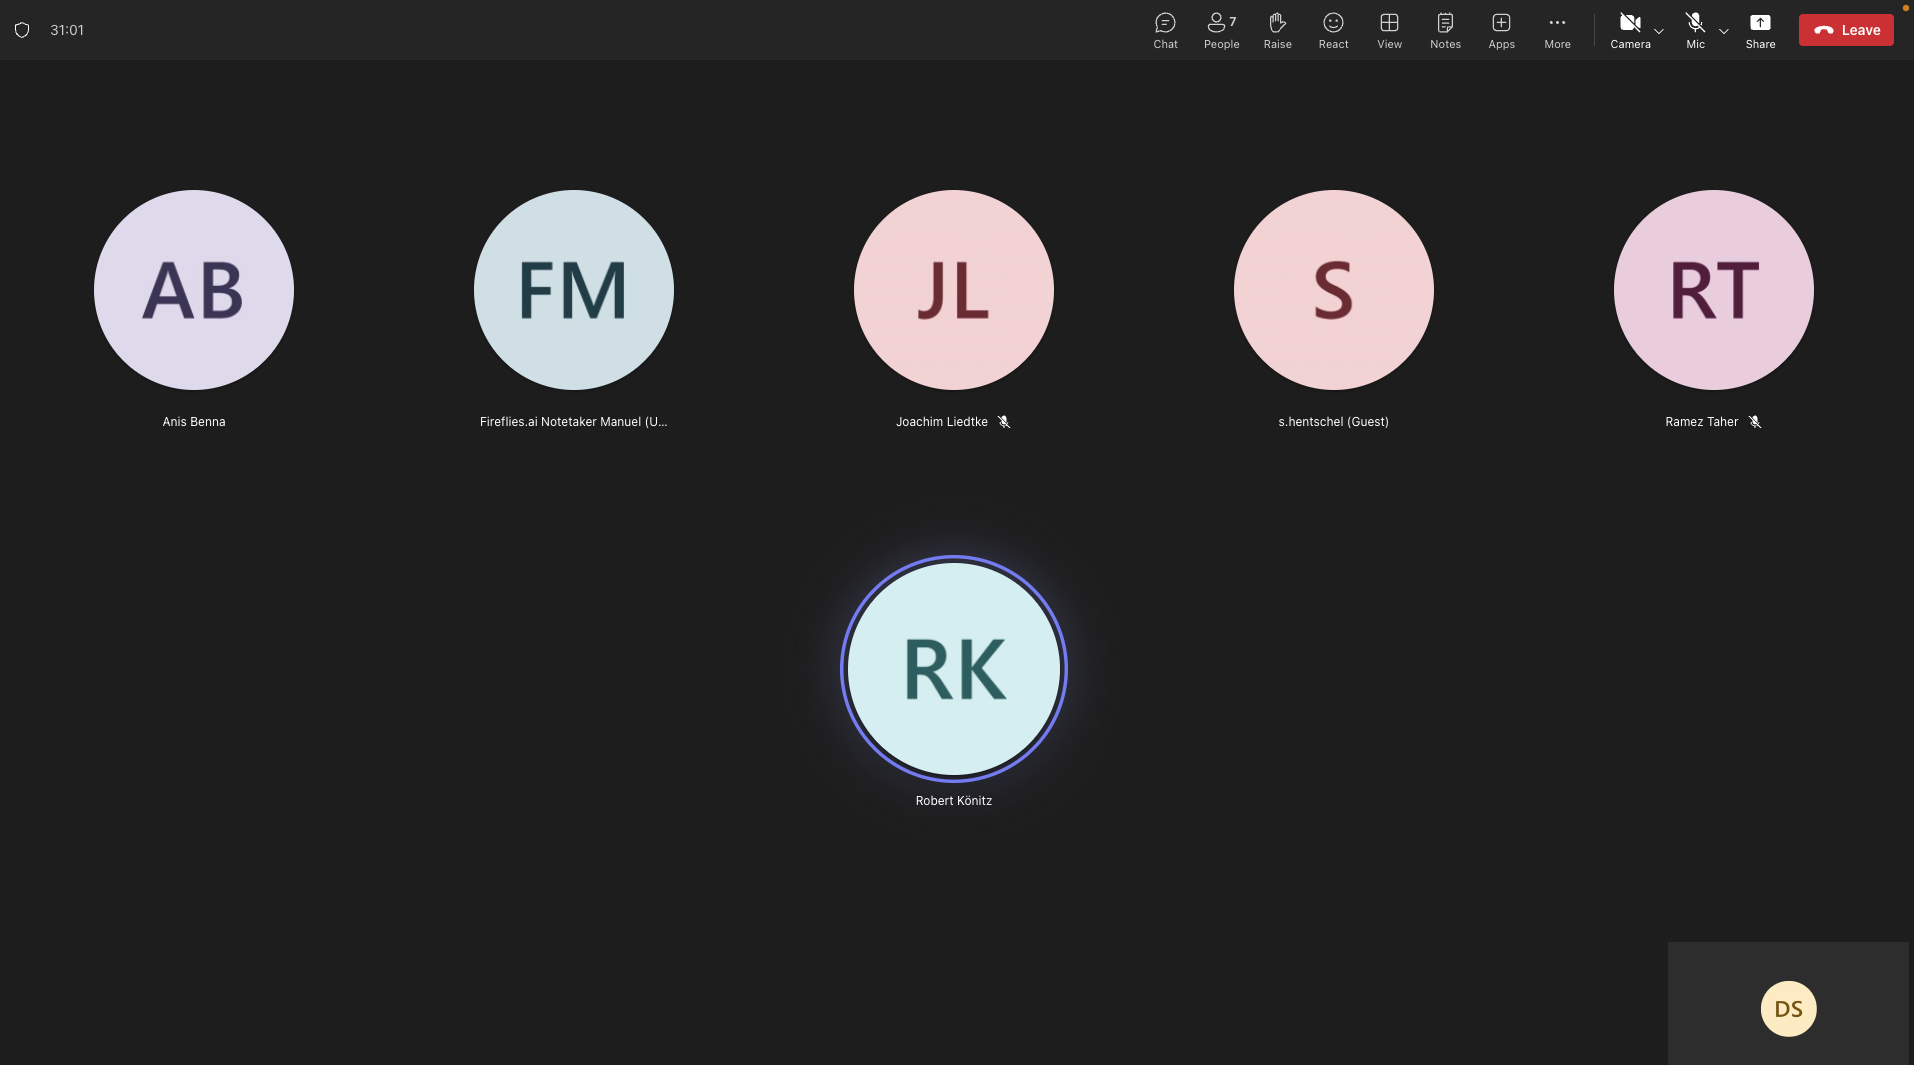
\includegraphics[width=0.9\textwidth]{src/assets/chapters/JF MEETING.png}
    \caption{Screenshot of Video Call with Client}
    \label{fig:client_meeting}
\end{figure}
\begin{figure}[H]
    \centering
    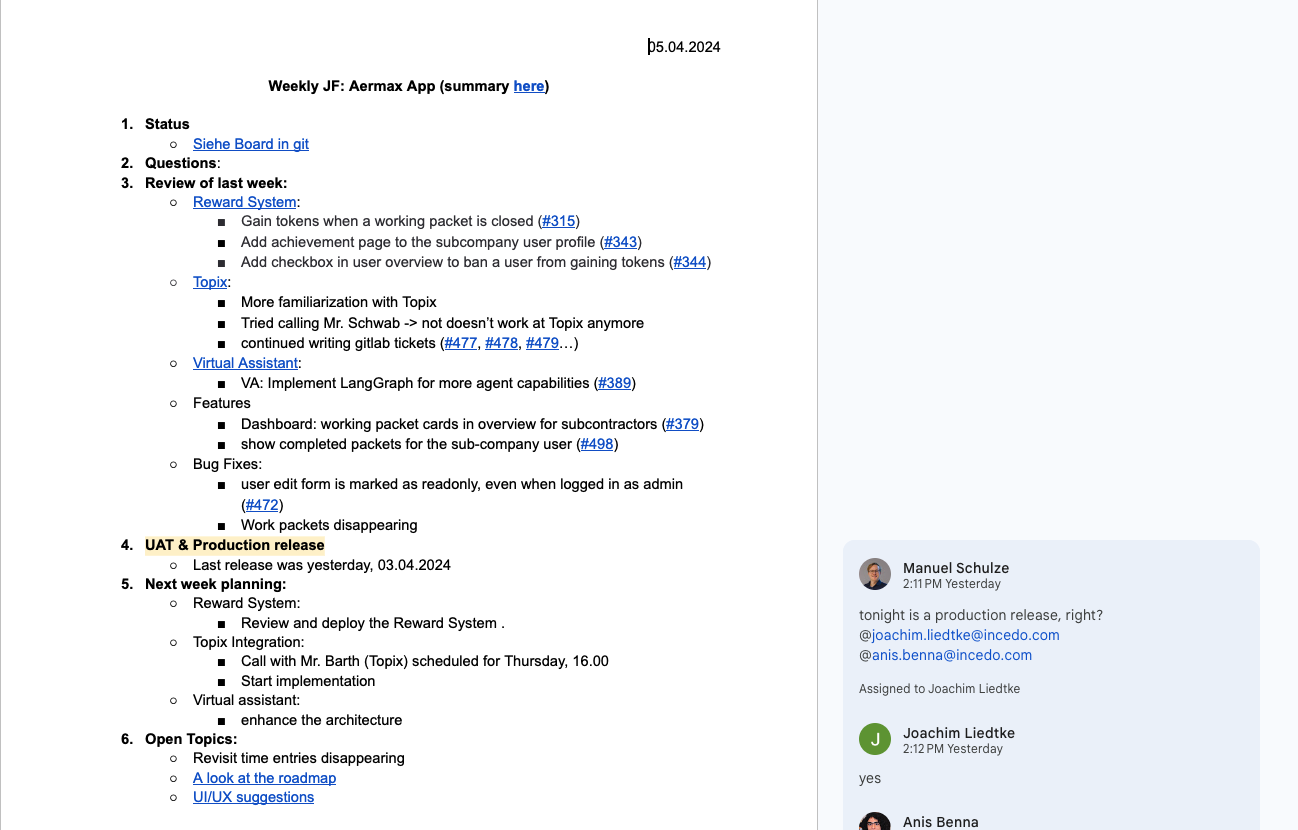
\includegraphics[width=0.9\textwidth]{src/assets/chapters/JF.png}
    \caption{ Weekly JF Meeting Summary Log for the Aermax App Project}
    \label{fig:Weekly_JF}
\end{figure}

\subsection{Ticket Management and Workflow}
\textbf{Tool:} Use of GitLab for managing tasks. \\
\textbf{Process:} Tickets are created, assigned, and tracked through stages like "To Do," "In Progress," "In Review," and "Done."
\begin{figure}[H]
    \centering
    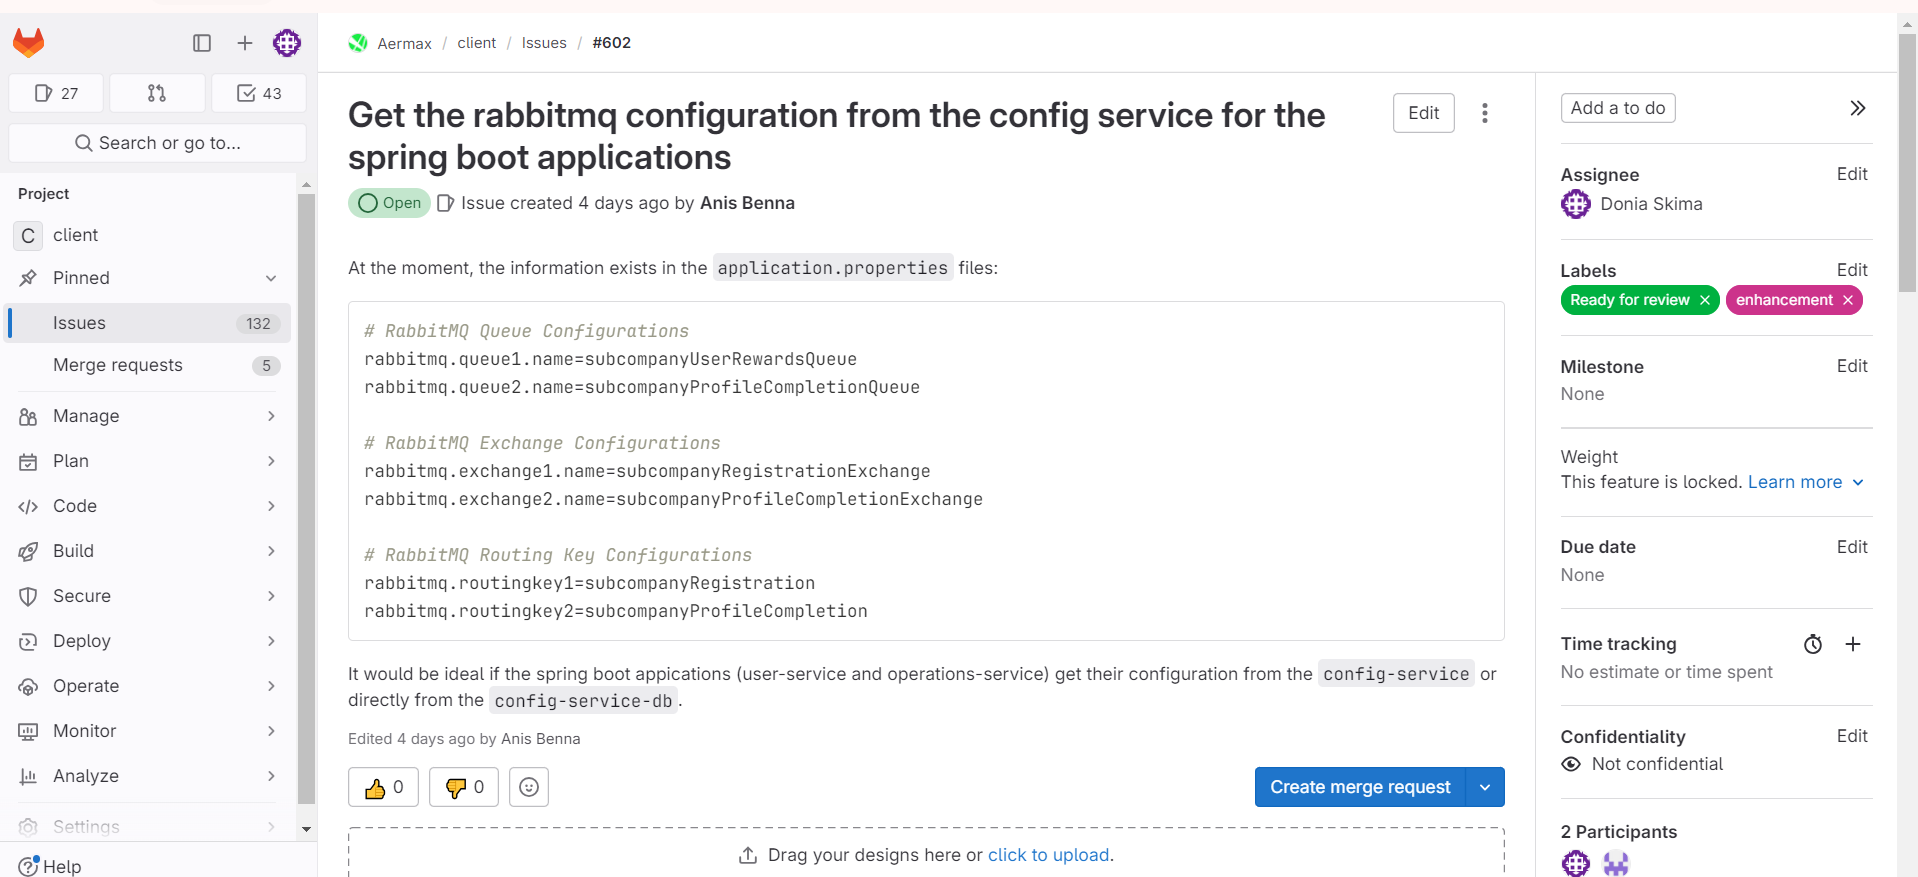
\includegraphics[width=0.9\textwidth]{src/assets/chapters/ticket.PNG}
    \caption{Example of Ticket in GitLab}
    \label{fig:ticket_management}
\end{figure}

\subsection{Communication Tools}
\textbf{Microsoft Teams:} For instant messaging. \\
\textbf{Microsoft Teams/Google Meet:} For video conferencing. \\
\textbf{Google Docs:} For documentation and collaborative editing.
\begin{figure}[H]
    \centering
    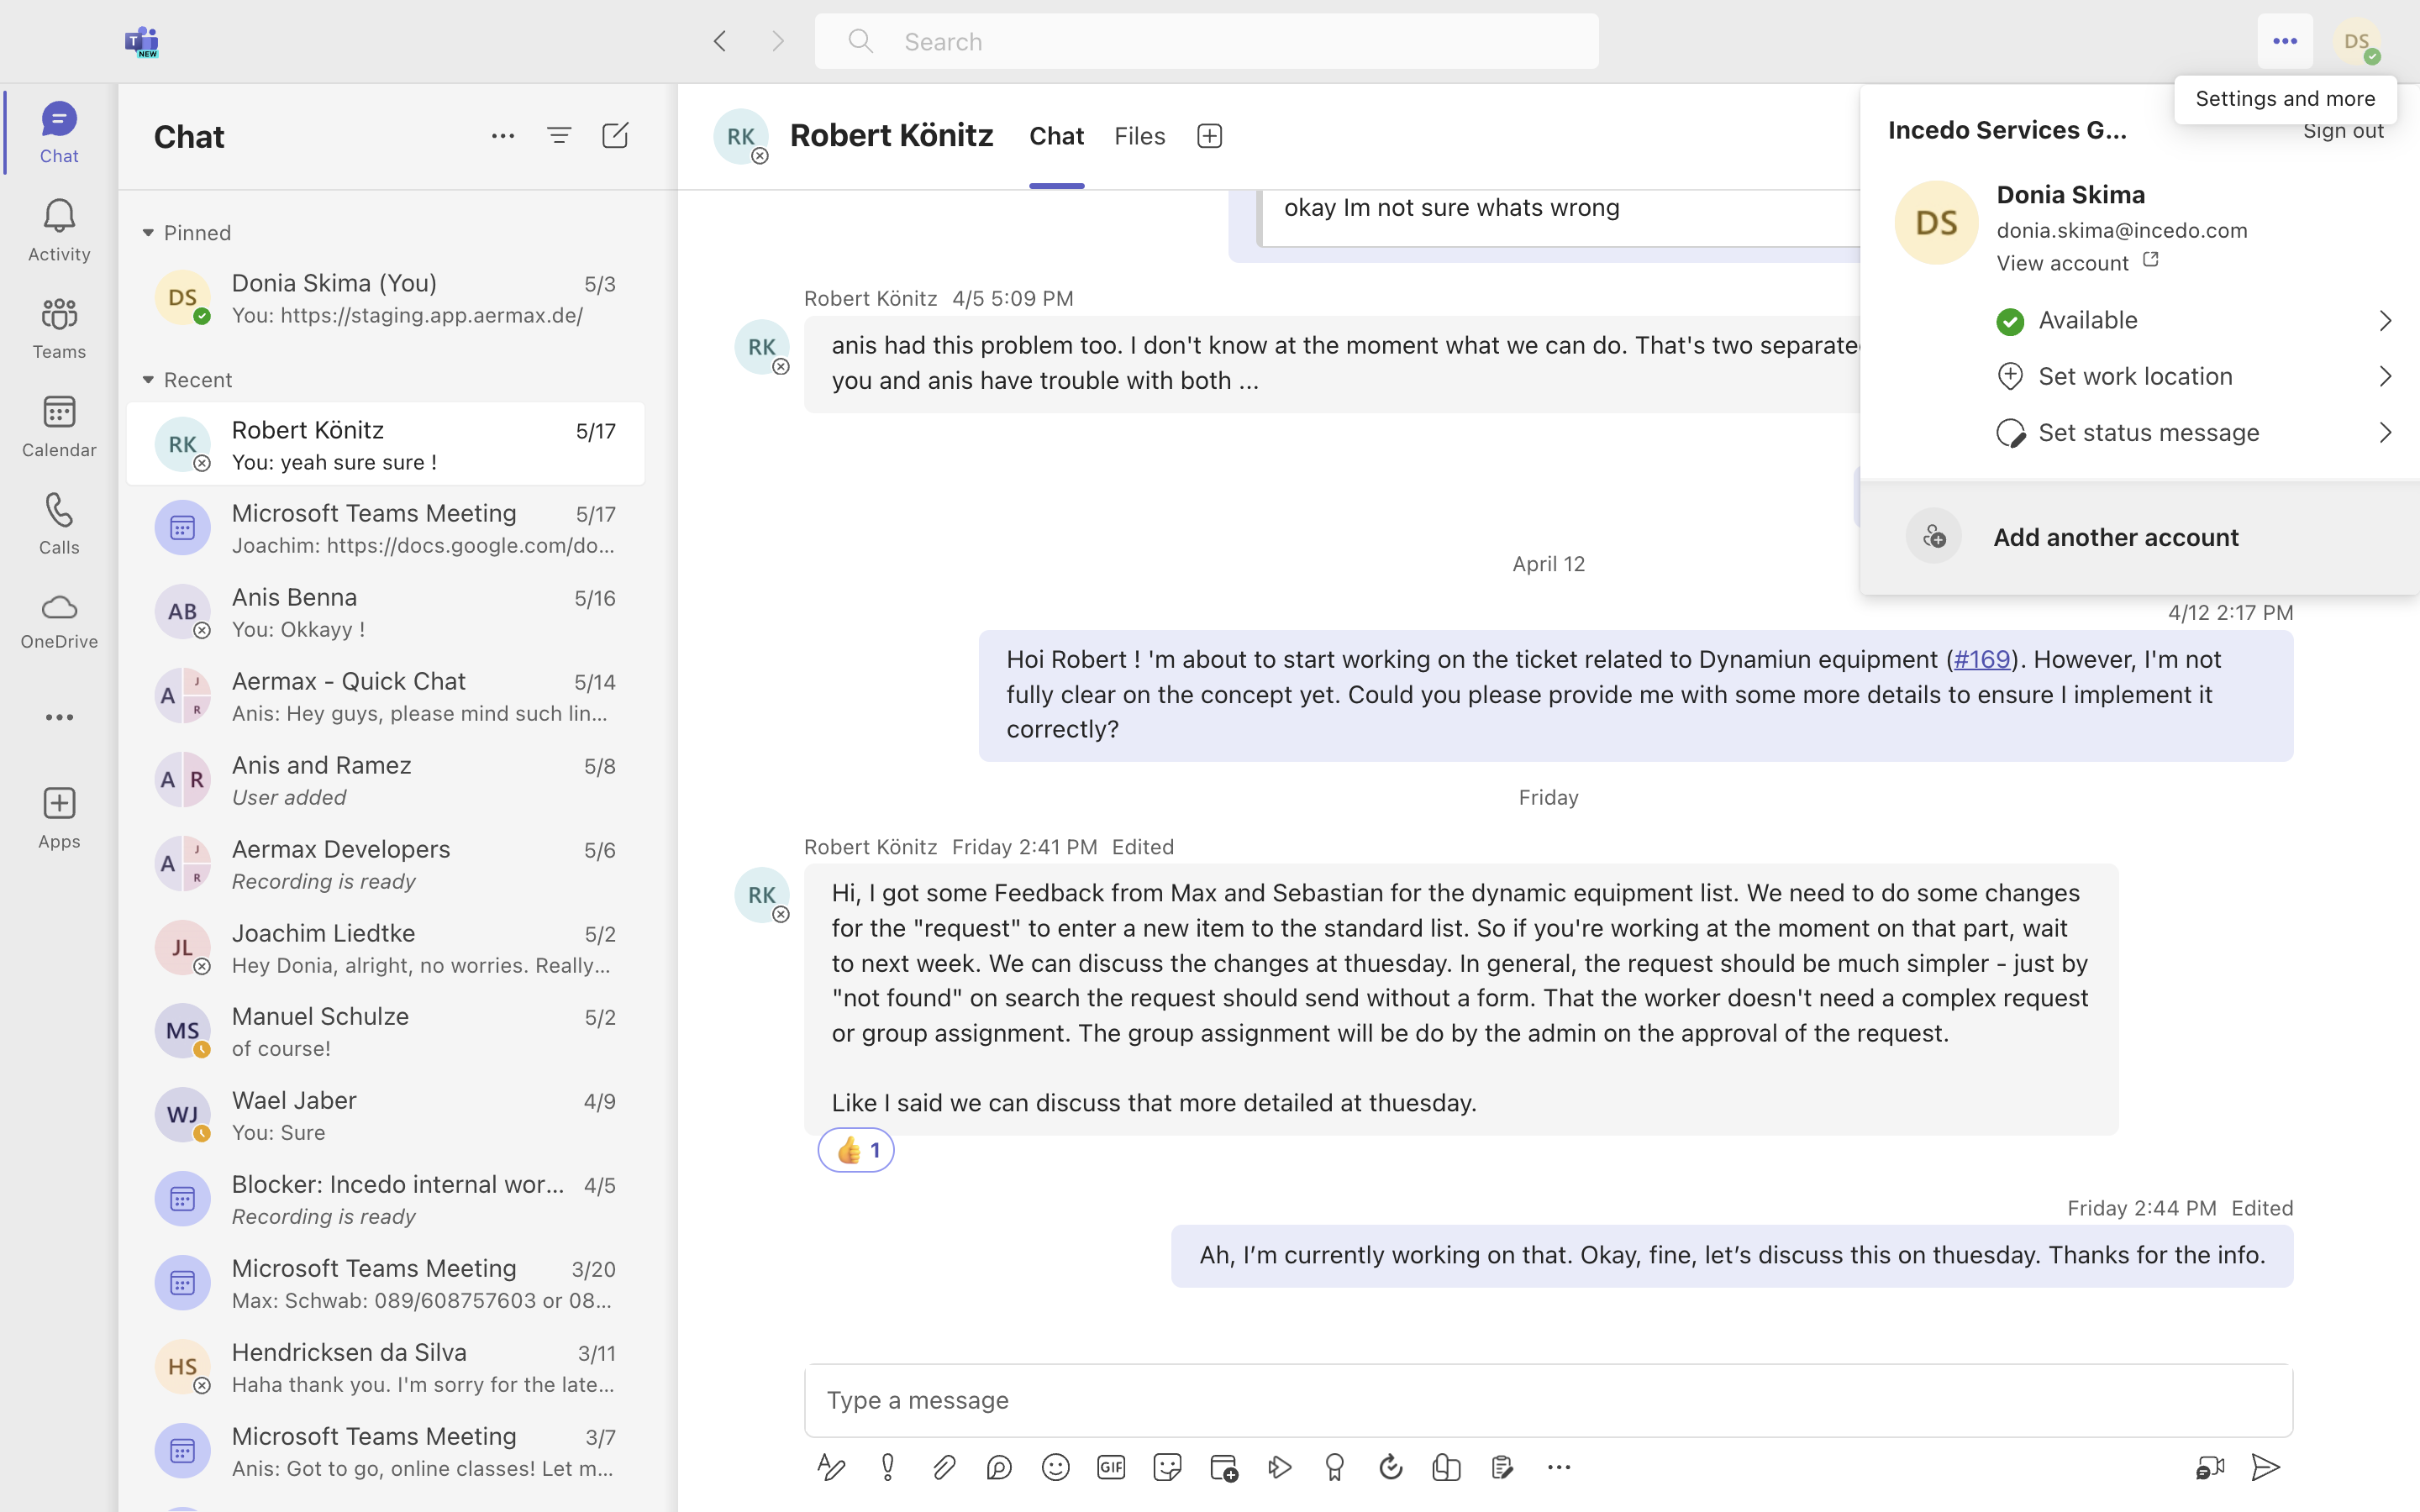
\includegraphics[width=0.9\textwidth]{src/assets/chapters/MicrosoftTeams.png}
    \caption{Screenshot of Microsoft Teams in Use}
    \label{fig:communication_tools}
\end{figure}

\section{Major Features and Enhancements}

\subsection{Sprint Backlog Detail}
Below is a detailed representation of our sprint backlog, showcasing the major tasks we committed to delivering in Sprint 1. We fixed around \textbf{26+ bugs, feature enhancements,} and new features in Sprint 1. Below, we're going to share some of them.

% Set up the longtable environment to break across pages
\begin{longtable}{|p{2.5cm}|p{2cm}|p{2.75cm}|p{1.75cm}|p{1.75cm}|p{1.25cm}|}

    % Table header information
    \caption{Detailed Sprint Backlog} \\
    \hline
    \textbf{Type} & \textbf{Title} & \textbf{Description} & \textbf{Priority} & \textbf{Assignee} & \textbf{Status} \\
    \hline
    \endfirsthead
    
    % Table continuation header information
    \multicolumn{6}{c}%
    {{\bfseries Table \thetable\ Continued from previous page}} \\
    \hline
    \textbf{Type} & \textbf{Title} & \textbf{Description} & \textbf{Priority} & \textbf{Assignee} & \textbf{Status} \\
    \hline
    \endhead
    
    % Footer at the end of each page (if needed)
    \hline
    \multicolumn{6}{|r|}{{Continued on next page}} \\ \hline
    \endfoot
    
    % Footer at the end of the table (if needed)
    \hline
    \endlastfoot
    
    % Table content
    Feature & Implement Self-Registration & Allow subcontractors to self-register on the platform. & High & Donia Skima & Done \\    \hline
    Enhancement & Adjust Feedback Notification & Update feedback functionality to include notifications in teams. & Medium & Ramez Taher & Done \\
    \hline
    Enhancement & Set Dynamic Project Status & Dynamically set project status based on packet statuses. & High & Donia Skima & Done \\
    \hline
    Enhancement & Add Field to User Edit & Include additional fields in the user edit form. & Medium & Donia Skima & Done \\
    \hline
    Feature & Set Default Calendar View & Remember last selection for default calendar view using localStorage. & Medium & Ramez Taher & Done \\
    \hline
    Enhancement & Restrict Project Creation & Prevent subcontractors from creating new projects. & High & Ramez Taher & Done \\
    \hline
    Enhancement & Remove Team Types & Remove unnecessary team types from the app to streamline functionality. & Low & Donia Skima & Done \\
    \hline
    Feature & Calendar View with New Filters & Implement new filters for the calendar view for better UX. & High & Ramez Taher & Done \\
    \hline
    Feature & Implement Google Maps URL Generation & Generate Google Maps URLs for address visualization in subcompany user view. & Medium & Donia Skima & Done \\
    \hline
    Bug & Overhaul User Access Restrictions & Fix critical access restrictions and bugs for subcompany users. & High & Donia Skima & Done \\
    \hline
    Feature & Overhaul the Role System & Revise the role system to clarify permissions and responsibilities. & High & Donia Skima & Done \\
    \hline
    Feature & Automate Username Generation & Auto-generate usernames during self-registration. & Medium & Donia Skima & Done \\
    \hline
    Feature & Remember Date Filters for Calendar & Implement a feature to remember date filters for the calendar. & Low & Ramez Taher & Done \\
    \hline
    Feature & Overhaul the Project Status & Update project status features and adjust status enums and filters. & High & Ramez Taher & Done \\
    \hline
    Bug & Fix Read-Only State of User Edit Form & Correct the issue with the user edit form being read-only for admins. & Medium & Donia Skima & Done \\
    \hline
    Bug & Remove Duplicate Aggregated Phases & Remove any duplicate instances of aggregated phases in the system. & High & Donia Skima & Done \\
    \hline
    Enhancement & Enhance Working Packets UI \& UX & Improve the UI and UX for working packets. & Medium & Ramez Taher & Done \\
    \hline
    Feature & Dynamic Equipment List & The ticket describes an issue with a dynamic equipment list system where equipment items are grouped and managed. & High & Donia Skima & Done \\
    \hline
    \end{longtable}
    \subsection{Dynamic Equipment List}
    \subsubsection{Previous Implementation}
    The Dynamic Equipment List feature was previously implemented as a static list. This static list required manual updates and did not reflect real-time changes to the equipment database. The key characteristics of the static implementation included:
    \begin{itemize}
        \item Manual updates to the equipment list.
        \item Limited flexibility and responsiveness to changes.
        \item High maintenance overhead due to frequent updates.
    \end{itemize}
    
    \subsubsection{Issues with Static Implementation}
    The static implementation had several drawbacks:
    \begin{itemize}
        \item \textbf{Scalability:} As the number of equipment items grew, maintaining the static list became increasingly cumbersome.
        \item \textbf{Real-time Updates:} Any changes to the equipment database were not immediately reflected in the list, leading to potential inconsistencies.
        \item \textbf{User Experience:} Users could not rely on the list for up-to-date information, which impacted their ability to make informed decisions.
    \end{itemize}
    
    \begin{figure}[H]
        \centering
        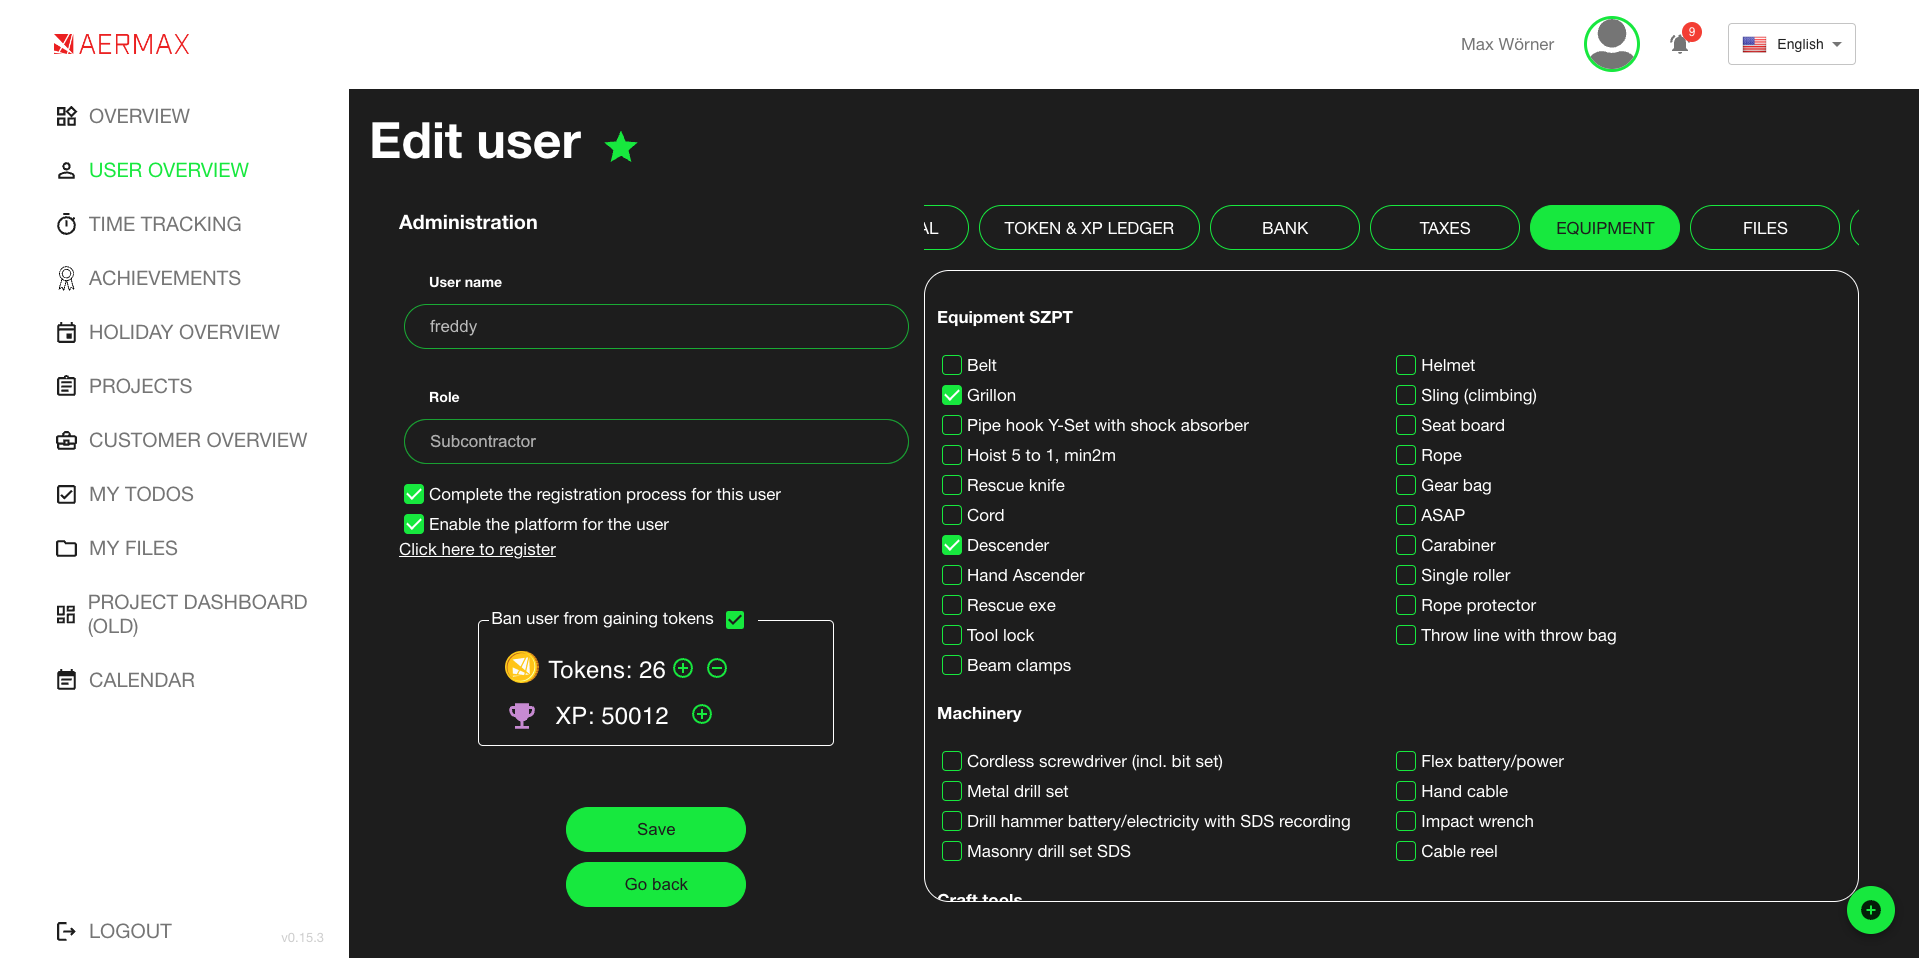
\includegraphics[width=0.9\textwidth]{src/assets/chapters/StaticDynamicEquipementList.png}
        \caption{Previous Static Equipment List}
        \label{fig:static_equipment_list}
    \end{figure}
    
    \subsubsection{Planned Dynamic Implementation}
    To address these issues, we are transitioning to a dynamic equipment list. The dynamic implementation will automatically update the list based on changes in the equipment database, ensuring real-time accuracy and reducing maintenance overhead. Key features of the dynamic implementation include:
    \begin{itemize}
        \item \textbf{Real-time Updates:} The list will automatically reflect changes made to the equipment database.
        \item \textbf{Improved Scalability:} The system can handle an increased number of equipment items without additional maintenance.
        \item \textbf{Enhanced User Experience:} Users will have access to up-to-date information, improving their ability to make decisions.
        \item \textbf{Reduced Maintenance:} Eliminates the need for manual updates, reducing the time and effort required to maintain the list.
    \end{itemize}
    
    \begin{figure}[H]
        \centering
        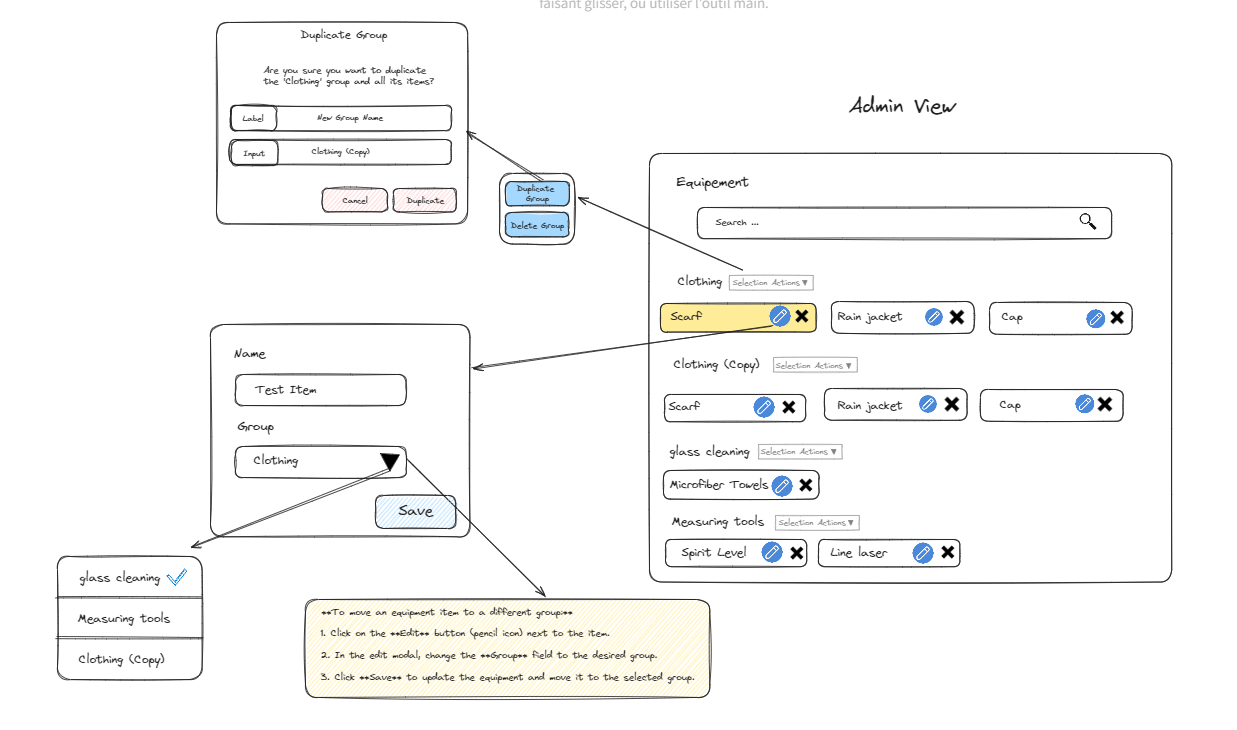
\includegraphics[width=0.9\textwidth]{src/assets/chapters/DynamicEquipementAdmin.PNG}
        \caption{Planned Dynamic Equipment List - Admin View}
        \label{fig:dynamic_equipment_list_admin}
    \end{figure}
    
    \begin{figure}[H]
        \centering
        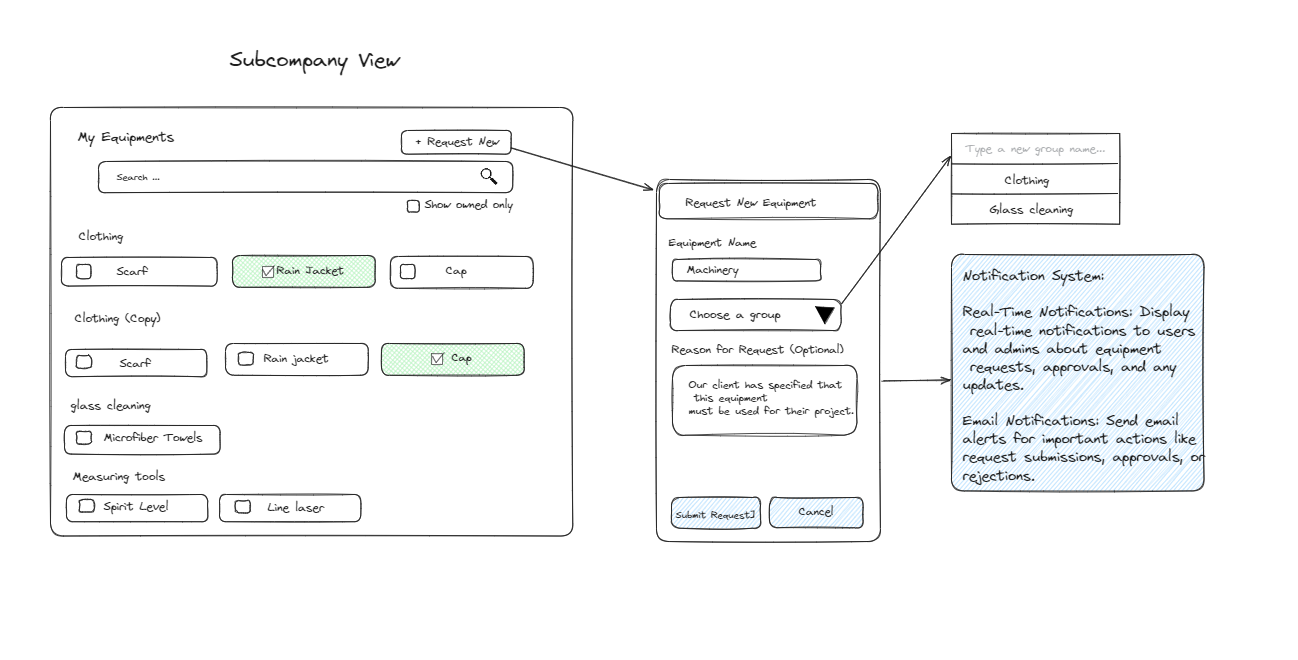
\includegraphics[width=0.9\textwidth]{src/assets/chapters/DynamicEquipementSubcompany.PNG}
        \caption{Planned Dynamic Equipment List - Subcompany View}
        \label{fig:dynamic_equipment_list_subcompany}
    \end{figure}
    \subsubsection{Conception of New Feature}
To effectively transition from a static to a dynamic equipment list, we need to carefully design the system architecture. The following sections provide a detailed overview of the class structure and interactions.

\paragraph{Class Diagram}
The class diagram below illustrates the key components and relationships involved in the dynamic equipment list feature.

 